\documentclass[pdftex,
a4paper,
11pt,
halfparskip % Removes the horizontal indet when starting a new paragraph.
]{scrartcl}   
%
%---------------------------------------------------
%----- Packages
%---------------------------------------------------
%
\usepackage[T1]{fontenc} 
\usepackage[utf8]{inputenc}
% This template is for english text only. You need to change it to German and adapt to your needs. We only provide English templates.
\usepackage[english]{babel}  
\usepackage{ae} 
\usepackage{fancyref} 
\usepackage{fancyhdr} % Define simple headings 
\usepackage{xcolor}
\usepackage{url}
\usepackage[pdftex]{graphicx}  
\usepackage{hyperref} % turn all your internal references into hyperlinks
\renewcommand{\sectionautorefname}{Section} %rename subsection to Section for better referencing

% ToDo List
\usepackage{enumitem,amssymb}
\newlist{todolist}{itemize}{2}
\setlist[todolist]{label=$\square$}
\usepackage{pifont}
\newcommand{\cmark}{\ding{51}}%
\newcommand{\xmark}{\ding{55}}%
\newcommand{\done}{\rlap{$\square$}{\raisebox{2pt}{\large\hspace{1pt}\cmark}}%
\hspace{-2.5pt}}
\newcommand{\wontfix}{\rlap{$\square$}{\large\hspace{1pt}\xmark}}

\definecolor{fu-orange}{RGB}{255,153,0}

% Fancy Tabellen
\usepackage{tabularx}
\definecolor{usethiscolorhere}{rgb}{0.92,0.92,0.92}
\definecolor{bamacolor}{RGB}{197, 210, 228}
\usepackage{booktabs}  
% own column Type Y!!!
\usepackage{ragged2e}  % for '\RaggedRight' macro (allows hyphenation)
\newcolumntype{Y}{>{\RaggedRight\arraybackslash}X}

% For the ganntchart
\usepackage{pgfgantt}
% a new command is defined that allows to include an empty page when needed

\usepackage{afterpage}

\newcommand{\blankpage}{
\newpage
\thispagestyle{empty}
\mbox{}
\newpage
}
%
%---------------------------------------------------
%----- PDF and document setup
%---------------------------------------------------
%
\hypersetup{
	pdftitle={<My title>},  % please, add the title of your thesis
    pdfauthor={<Author>},   % please, add your name
    pdfsubject={<<Bachelor thesis>, Institute of Computer Science, Freie Universität Berlin>}, % please, select the type of this document
    pdfstartview={FitH},    % fits the width of the page to the window
    pdfnewwindow=true, 		% links in new window
    colorlinks=false,  		% false: boxed links; true: colored links
    linkcolor=red,          % color of internal links
    citecolor=green,        % color of links to bibliography
    filecolor=magenta,      % color of file links
    urlcolor=cyan           % color of external links
}
%
%---------------------------------------------------      
%----- Settings for word separation  
%---------------------------------------------------      
% Help for separation (from package babel, section 22)):
% In german package the following hints are additionally available:
% "- = an explicit hyphen sign, allowing hyphenation in the rest of the word
% "| = disable ligature at this position. (e.g., Schaf"|fell)
% "~ = for a compound word mark without a breakpoint (e.g., bergauf und "~ab)
% "= = for a compound word mark with a breakpoint, allowing hyphenation in the composing words
% "" = like "-, but producing no hyphen sign (e.g., und/""oder)
%
% Describe separation hints here:
\hyphenation{
% Pro-to-koll-in-stan-zen
}

%---------------------------------------------------      
%----- Settings for title page 
%---------------------------------------------------

\begin{titlepage}

 
\title{
% TODO: Select the type of the thesis proposal you are writing.
% Source: https://degree.studentnews.eu/
{\normalsize --<B. Sc. / M. Sc.> Thesis Proposal\footnote{Template Version 2.0 --- 2021-07-14}--\\
% TODO: The title should be capitalized. If unsure use the following website: https://capitalizemytitle.com/
[4ex]
{\LARGE<Working Title of Your Thesis>}\\ 
[4ex]
\small Freie Universität Berlin\\Institute of Computer Science}\\
{\small Human-Centered Computing (HCC) Research Group}\\
[2ex]
}

\author{
% TODO: Add your full name here.
{\normalsize<First name Last name>}\\
% TODO: Add your matriculation number!
{\normalsize Student Number: <Your matriculation number>}\\
% TODO Please use the email address provided by FU Berlin.
{\normalsize <firstname.lastname@fu-berlin.de>}\\
% TODO: Add the date. This is important, since there will be different versions of you proposal.
{\normalsize Date of Proposal Submission: <Month, DD, YYYY>}\\
% TODO: Please add the version, so we can keep track of the number of iterations.
{\normalsize Version: <\#>}\\\\

\rule{\textwidth}{0.4pt}\\
\\
{\normalsize Supervisor:\\
% TODO: Add the name of your supervisor.
\normalsize<First name Last name>\footnote{Department of Mathematics and Computer Science, Human-Centered Computing Research Group}, Freie Universität Berlin, Germany}\\\\

{\normalsize Examiner:\\
\normalsize Prof. Dr. Claudia Müller-Birn\footnote{Department of Mathematics and Computer Science, Human-Centered Computing Research Group}, Freie Universität Berlin, Germany\\
% TODO: Add the name of your second reviewer.
\normalsize <Prof. Dr. Second Examiner\footnote{Department of Mathematics and Computer Science, <Name of Research Group>}>, Freie Universität Berlin, Germany}\\\\
}

\date{} % This omits the date on the title page.

\end{titlepage}

%---------------------------------------------------      
%----- Setting up your document 
%---------------------------------------------------

\begin{document}

\maketitle
\thispagestyle{empty} % remove page number on the title page

%---------------------------------------------------
%----- GUIDELINES - Please remove this part before handing in your expose.
%---------------------------------------------------
\pagecolor{fu-orange}

\section*{Guidelines}
\emph{Please remove this section before handing in your proposal.}

You should plan 3--4 feedback rounds for finalizing your proposal.
Before handing in the proposal to your supervisor, please check if your proposal fulfills the following criteria:

\begin{todolist}
  \item A proposal for a B. Sc. thesis should have about five pages of text. Excluding the title page, timeline, references, and outline.
  \item A proposal for an M. Sc. thesis should have a maximum of 10--20 pages.
  \item Your proposal has to include a research question. The research question has to be in the form of a sentence ending with a question mark.
  \item Include the assumed deadline for submitting your thesis in the timeline.
  \item Define a short, significant title that reflects the contents of your thesis. Please note, you can change the title in the final version.
  \item Use American English, for example, instead of vi\textbf{s}ualisation (BE) $\rightarrow$ visuali\textbf{z}ation (AE).
  \item You can write the proposal and also the final thesis either in German or in English. However, we recommend English. If you use German, please adapt the latex template on your own.
  \item The proposal should be comprehensible, so that not only specialists can understand it.
  \item Use correct spelling and grammar, as well as correct scientific language.
  \item Use the ACM citation style.
  \item Avoid any indication of possible plagiarism. Please remember, in severe cases, plagiarism results in a fail.
 
\end{todolist}

\subsection*{Where to find literature?}
Be aware that the Human-Centered Computing (HCC) Research Group conducts research in the areas of Human-Computer Interaction (HCI) and Collaborative Computing. Therefore, articles from the following conferences are of particular interest\footnote{Upcoming conference are listed on the website of the ACM Special Interest Group on Computer-Human Interaction (CHI): \url{https://sigchi.org/conferences/upcoming-conferences/}}: 

\begin{itemize}
    \itemsep0em % This should move to the global layout section.
    \item CHI --- Human Factors in Computing Systems
    \item CSCW --- Computer Supported Cooperative Work
    \item IUI --- International Conference on Intelligent User Interfaces
    \item DIS --- Designing Interactive Systems Conference
\end{itemize}

You can find the publications of these conferences in the Digital Library of ACM\footnote{ \url{https://dl.acm.org/}}. We highly recommend this search engine, as opposed to using the general search engine Google Scholar\footnote{\url{https://scholar.google.com/}}. In ACM, the papers are already contextualized (by considering the respective conference in the search filters), and thus, you ensure that the work is relevant. If you have any doubts, talk to your supervisor.

\subsection*{What is a human-centered design approach?}
At HCC Research Group, we always apply a human-centered design (HCD) approach. This approach is taught in the \emph{Human-Computer Interaction I} course. If you are not familiar with this approach, you need to learn it before starting your thesis. Please contact your supervisor to get access to the slides and videos of the course. In order to reach your goals, you have to make sure that you understand which research methods are most suitable to fulfill your goals. We recommend reviewing available methods and their practical application in the field of HCI~\cite{lazar2017research, olson2014ways}. Both mentioned sources and additional books are available at the HCC Research Group's library\footnote{We also set up an open Zotero library where we share literature references that have shown to be helpful in prior theses regarding fundamental knowledge on HCI methods. You can find the open Zotero library ''HCC --- Thesis Literature'' here: \url{https://www.zotero.org/groups/2815440/hcc_-_thesis_literature}.}. Please talk to your supervisor.


\afterpage{\nopagecolor}

%---------------------------------------------------
%----- Summary
%---------------------------------------------------
\section*{Summary}
Summarize your thesis project in 150 words (in English).

\section*{Zusammenfassung}
Summarize your thesis project in 150 words (in German).

%---------------------------------------------------
%----- Contents
%---------------------------------------------------
\tableofcontents

 % page number is set to "1" otherwise it would be "3"
\setcounter{page}{1}

%---------------------------------------------------      
%----- CONTENT PART 
%---------------------------------------------------
%---------------------------------------------------
%----- Introduction
%---------------------------------------------------
%************************************************************************
\section{Introduction}
\label{sec:introduction}
% Introduction to the topic.
% Explain why this work is important giving a general introduction to the subject,
% list the basic knowledge needed and outline the purpose of the report. 
%************************************************************************
This section should start with a short thematic introduction of your planned thesis. This includes a description of the context of your thesis, your subject area, and the domain or field in which you aim to do your research. 

In ~\autoref{subsec:motivation} you describe the motivation of your research, why it is relevant, and in ~\autoref{subsec:goal}, you specify the overarching aim of your thesis.

\begin{table}[h]
\small
\colorbox{usethiscolorhere}{
\centering
\begin{tabularx}{\textwidth}{@{} r Y @{}}
	&
	\textbf{Examples}\vspace{2mm}\\
    \textbf{Context} & Machine Learning \vspace{2mm}\\
	\textbf{Subject area} &	Explanations \vspace{2mm}\\
    \textbf{Domain or application area} & Medicine \vspace{2mm}\\
    \textbf{Field of Research} & HCI \vspace{2mm}\\
\end{tabularx}
}
\end{table}

%************************************************************************
\subsection{Motivation}
\label{subsec:motivation}
% Motivation and relevance of the topic.
%************************************************************************
In this section, you should motivate why the problem you are tackling matters and why this is relevant. You want to give the reader enough background knowledge to understand your problem in order to understand your approach. Therefore, introduce the reader to all the necessary fields your research question is part of. Give an overview of why this is interesting. Please illustrate your problem by using an example.

%************************************************************************
\subsection{Goal}
\label{subsec:goal}
% Gap you want to close with your research.
% Goal of your work.
% Your research question.
% List the main research question(s) you want to answer.
% Explain whether your research will provide a definitive answer or simply contribute towards an answer
%************************************************************************
This part of the expose is the most important one since you have to specify the objectives~(goal) of your thesis. The goal of your thesis should be as specific as possible. You also need to outline \emph{what} contribution you are making and \emph{where} you want to make a contribution. By \emph{where} we mean which field of research. Please make sure that the goals are realistic and that you are able to evaluate your goals. Please list the main research question(s) you want to answer. Explain whether your research will provide a
definitive answer or simply contribute towards an answer.

\begin{table}[htb]
\small
\colorbox{bamacolor}{
\centering
\begin{tabularx}{\textwidth}{@{} r Y @{}}
	&
	\textbf{Distinction between Bachelor and Master theses}\vspace{2mm}\\
    \textbf{B. Sc. Thesis} &
    For a B. Sc. thesis, the actual implementation is often a goal. Therefore a thoughtful application of the HCD approach~\cite{gulliksenKeyPrinciplesUsercentred2003, dis20109241} is sufficient. \vspace{2mm}\\
	\textbf{M. Sc. Thesis} &
	In the case of a M. Sc. thesis, a scientific objective needs to be clearly stated and a scientific contribution has to be made. According to \cite{contributionTypes2016} there are seven different contribution types in HCI: theoretical, methodological, empirical, artifact, dataset, survey, and opinion contribution.\vspace{2mm}\\
\end{tabularx}
}
\end{table}

\begin{table}[htb]
\small
\colorbox{usethiscolorhere}{
\centering
\begin{tabularx}{\textwidth}{@{} r Y @{}}
	&
	\textbf{M. Sc. Example taken from ~\cite{Uga1324610}}\vspace{2mm}\\
    \textbf{Goal} & Explore how trustworthy AI can be designed: The goal of this thesis is to suggest design guidelines for the development of trust-inducing explanations to AI-based prediction systems. \vspace{2mm}\\
	\textbf{Contribution} &	Guidelines for designers, that can be applied in a variety of contexts.\vspace{2mm}\\
	\textbf{Contribution Type} & Empirical \vspace{2mm}\\
    \textbf{Research Question} & How can AI predictions be articulated to be trustworthy and actionable?\\
    Sub-questions & --- What explanatory aspects are important to support trust?\\
    & --- What guidance should the articulation provide towards actions to take?\\
    & --- Which presentation formats best support formation of trust?\vspace{2mm}\\
	\textbf{Methodology} & Research through design \vspace{2mm}\\
\end{tabularx}
}
\end{table}

\begin{table}[htb]
\small
\colorbox{usethiscolorhere}{
\centering
\begin{tabularx}{\textwidth}{@{} r Y @{}}
	&
	\textbf{B. Sc. Example taken from~\cite{Joppien2020}}\vspace{2mm}\\
    \textbf{Goal}
    & The goal is to make the diversity of equally valid dimensionality reduction outputs comprehensible through a variety of results so that an individual can make an informed decision. \vspace{2mm}\\
	\textbf{Contribution}
	& -\vspace{2mm}\\
    \textbf{Research Question}
    & Which visual similarity measures help non-technical experts (especially
in the specific scenario described later) to\\
    Sub-questions
    & --- grasp the entire space of possible dimensionality reduction outcomes?\\
    & --- successfully find the most useful visual representation of the information needed for their task?\\
	\textbf{Methodology}
	& HCD\vspace{2mm}\\
\end{tabularx}
}
\end{table}
%---------------------------------------------------
%----- Background
%---------------------------------------------------
%************************************************************************
\section{Background}
\label{sec:background}
% List relevant work by others,
% or preliminary results you have achieved with a detailed and accurate
% explanation and interpretation.
% Include relevant photographs, figures or tables to illustrate the text.
% This section should frame the research questions that your subsequent research will address. 
%************************************************************************
Please add a sentence that summarizes what this section is about and what the reader can expect.
%************************************************************************
\subsection{Context of the Project and Problem Description} 
\label{sec:context}
%************************************************************************
Explain all the surroundings that are necessary to understand the broader context of your work. If necessary, give a brief introduction to non-HCI research literature as background knowledge. It is best to include a specific scenario\footnote{Scenarios are defined as an \emph{''informal narrative description''}~\cite{carrol1999five}. \emph{''It describes human activities or tasks in a story that allows exploration and discussion of contexts, needs, and requirements. It does not necessarily describe the use of software or other technological support used to achieve a goal. Using the vocabulary and phrasing of users means that scenarios can be understood by stakeholders, and they are able to participate fully in development.''}~\cite{preeceInteractionDesignHumancomputer2015}.}. If you are designing a piece of software or graphical user interface, please specify your users and the tasks the users want to perform with your software.

%************************************************************************
\subsection{Related Work}
\label{sec:relatedwork}
%************************************************************************
This section consists of a literature review to situate your thesis in the scientific context. Which academic articles exist in your problem area, and how are they related to your work? When placing your thesis in the context of others, you need to consider other work, which uses a similar methodology or articles, who try to answer similar research questions.

\begin{table}[htb]
\small
\colorbox{bamacolor}{
\centering
\begin{tabularx}{\textwidth}{@{} r Y @{}}
	&
	\textbf{Distinction between Bachelor and Master thesis}\vspace{2mm}\\
    \textbf{B. Sc. Thesis} &
    A small literature review is mandatory, starting with the papers your supervisor provides. The related work part can also include a mini similiar tool analyzis if you are implementing a specific part of a software. \vspace{2mm}\\
	\textbf{M. Sc. Thesis} &
	A literature review is mandatory. If it is part of your project to choose a specific framework, then you need to conduct a short survey on existing frameworks. This also applies if you want to choose an algorithm to perform a specific task or want to design a study. \vspace{2mm}\\

\end{tabularx}
}
\end{table}

In the thesis announcement\footnote{Thesis announcements are descriptions for ''Open Theses'' on the HCC website: \url{https://www.mi.fu-berlin.de/en/inf/groups/hcc/theses/open/index.html}} already, relevant literature is provided. If this is not the case, please ask your supervisor for articles. Describing the state of the art is essential to identify the gap you would like to fill. Thus, the literature's description should clearly result in research gaps that lead to specific research questions. 


%************************************************************************
\subsection{Research Questions}
\label{subsec:question}
% Based on your overarching goal and the reviewed research, specify your research question.
%************************************************************************
In this section, you should name your research questions. Your research question should be based on the observation that prior research has a gap and some misconception. You can use words such as \emph{but} or \emph{however} to indicate this. Make sure that your emphasize the significance of your research. 
%---------------------------------------------------
%----- Your methodology approach
%---------------------------------------------------
%************************************************************************
\section{Methodology}
\label{subsec:methodology}
% Explain the methods and techniques which will be used for your project depending on the subject: field work, laboratory work, modeling technique, interdisciplinary collaboration, data type, data acquisition, infrastructure, software, etc.
%************************************************************************
Specify the overall methodology you want to apply in order to reach your goals and answer your research questions. We often apply the HCD process (cf.~\autoref{fig:hcd}): 1. Vision, 2. Analyze, 3. Design for Usability, 4. Construct and Deploy (Implementation), 5. Evaluate in Context, 6. Feedback. There is no predefined ready-to-use HCD process. You need to adapt the general process presented to your project. This means you need to think of specific methods in each step of the process. Please link your planned procedure to your goals. If your thesis follows a data science workflow, please adapt your methodology accordingly. It is not necessary to go through all the phases of the design process in detail, it is also possible to limit the number of iterations or focus on one particular phase. This depends on your project.

This chapter explains what method was chosen in the HCD process and why it helps to answer your research question.

\begin{figure}[h]
  \centering
  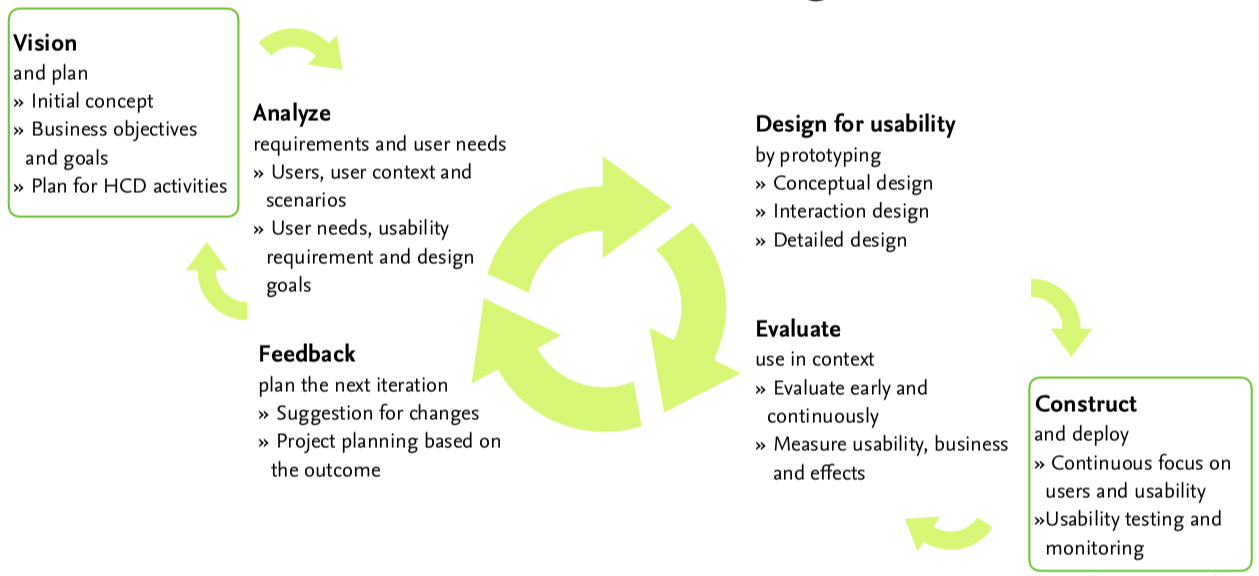
\includegraphics[width=\linewidth]{pics/hcd.png}
  \caption{User-centered System Design process by~\cite{gulliksenKeyPrinciplesUsercentred2003}}
\end{figure}

\begin{table}[htb]
\small
\colorbox{bamacolor}{
\centering
\begin{tabularx}{\textwidth}{@{} r Y @{}}
	&
	\textbf{Distinction between Bachelor and Master Thesis}\vspace{2mm}\\
    \textbf{B. Sc. Thesis} &
    The implementation phase is mandatory. \vspace{2mm}\\
	\textbf{M. Sc. Thesis} &
	The evaluation phase is mandatory. \vspace{2mm}\\

\end{tabularx}
}
\end{table}

Briefly describe the relevant planned steps of your HCD process in the following sections.

\subsection{Analyze}
\label{subsec:analyze}

\subsection{Design for Usability}
\label{subsec:design}

\subsection{Construct (Implementation)}
\label{subsec:implementation}

Especially in a B. Sc. thesis, an important part is the description of the technical concept. Even though in the proposal, this cannot be done in detail, the main libraries and the general architecture of the application should be outlined. Please use diagram types from the Unified Modeling Language (UML)\footnote{For further information, please check \url{https://en.wikipedia.org/wiki/Unified_Modeling_Language}.} for these details.

\subsection{Evaluation}
\label{subsec:evaluation}
%---------------------------------------------------
%----- Preliminary schedule and planned milestones
%---------------------------------------------------
\section{Project Plan}
\label{sec:plan}

It is useful to understand a Bachelor and Master thesis as a project. Projects are based on a plan, and each plan needs milestones\footnote{By milestone we mean a collection of tasks, which need to be finished by a specific date. You can also call it a work package.} and a timeline. Thus, in this section, you will break down your thesis project into manageable and specific milestones to realistically estimate the time you need. Especially if you use methods for the first time, we recommend to discuss this timeline with your supervisor. Please describe each milestone, what do you exactly do in that phase, in what order, what is the result or outcome of each step, and how does it contribute towards the goal of your thesis. As a result, you will outline a detailed timeline for your upcoming research.

According to the exam regulations: a Bachelor thesis\footnote{Please read \S~10 of the Study and Examination regulations for the bachelor’s degree program: \url{https://www.imp.fu-berlin.de/fbv/pruefungsbuero/Studien--und-Pruefungsordnungen/StOPO_BSc_Inf_-2014.pdf}, accessed May 16, 2021} takes about 360~hours (12~LP) and a Master thesis\footnote{Please read \S~9 of the Study and Examination regulations for the master’s
degree program: \url{https://www.imp.fu-berlin.de/fbv/pruefungsbuero/Studien--und-Pruefungsordnungen/STOPO_MSc_-Inf_-2014.pdf}, accessed May 16, 2021} is calculated with 900~hours (30~LP).

\begin{table}[h]
\small
\colorbox{usethiscolorhere}{
\centering
\begin{tabularx}{\textwidth}{@{} r Y @{}}
	& \begin{todolist}
  \itemsep0em % This should move to the global layout section.
  \item Calculate the hours you can effectively work on your thesis per week.
  \item Write down the planned date of handing in your thesis.
  \item Include up to 40~\% buffer in case of unforeseen problems (e.g., sickness, vacation).
  \item Include a Gantt-Chart.
\end{todolist}\\
    
\end{tabularx}
}
\end{table}




\subsection{Milestones}
\label{subsec:milestone}
Specify the milestones of your upcoming project. Please describe when you plan to achieve which milestone and what artifact(s) or outcome will result from each milestone. Also, keep in mind what the goal of each milestone is.


\begin{table}[h]
\small
\colorbox{usethiscolorhere}{
\centering
\begin{tabularx}{\textwidth}{@{} r Y @{}}
	\textbf{M1}
	& \textbf{Milestone --- Literature Review}\vspace{2mm}\\
	\textbf{Due date} & 2021-05-26 (Week $2$)\vspace{2mm}\\
     \textbf{Tasks} & Identifying and read other studies/thesis/papers evaluating the usability of chatbots in a medical context\vspace{2mm}\\
    \textbf{Outcome} & A list of relevant papers (e.g. folder in Zotero).\\
    & A written summary for each paper.\\
    & A final text summarizing the main findings and approaches, which might be useful for my project. \vspace{2mm}\\
    \textbf{Goal} & General understanding of methods to evaluate the usability of chatbots in the medical context. Having a good foundation for discussing my results in the context of other people's work.\vspace{2mm}\\
    
\end{tabularx}
}
\end{table}

\begin{table}[h]
\small
\colorbox{usethiscolorhere}{
\centering
\begin{tabularx}{\textwidth}{@{} r Y @{}}
	\textbf{M2}
	& \textbf{Milestone --- Evaluate Wikipedia's Advanced Search Interface}\vspace{2mm}\\
	Due date & 2021-06-15 (Week $4$)\vspace{2mm}\\
     Tasks & Prepare, conduct, and evaluate a remote usability test with four participants.\vspace{2mm}\\
    Outcome & Moderator script for conducting the usability test.\\
    & Affinity diagram with thematic clusters and headlines.\\
    & A list of usability issues sorted by severity.\vspace{2mm}\\
    Goal & Understanding the drawbacks of the current Wikipedia advanced search in order to (re)design a new interface.\vspace{2mm}\\
    
\end{tabularx}
}
\end{table}

\begin{table}[h]
\small
\colorbox{usethiscolorhere}{
\centering
\begin{tabularx}{\textwidth}{@{} r Y @{}}
	\textbf{M...}
	& \textbf{Milestone ---  ...}\vspace{2mm}\\
    Due date & \mbox{} \vspace{2mm}\\
    Tasks & \mbox{} \vspace{2mm}\\
    Outcome & \mbox{} \vspace{2mm}\\
    Goal & \mbox{} \vspace{2mm}\\
\end{tabularx}
}
\end{table}

\begin{table}[h]
\small
\colorbox{usethiscolorhere}{
\centering
\begin{tabularx}{\textwidth}{@{} r Y @{}}
	\textbf{M5}
	& \textbf{Milestone ---  High-Fidelity Prototype}\vspace{2mm}\\
	Due date & 2021-08-15 (Week $15$)\vspace{2mm}\\
     Tasks & Implement the final design and the main features with HTML and CSS. \vspace{2mm}\\
    Outcome & Repository with code and data on GitLab.\\
    & Deployed on Heroy and public link.\vspace{2mm}\\
    Goal & Interactive prototype, which is deployed and ready for testing.\vspace{2mm}\\
\end{tabularx}
}
\end{table}

\clearpage
\subsection{Timeline}
\label{subsec:timeline}
Now you need to transfer the milestones into a timeline. The time for your thesis will help you to set realistic time goals and maybe reconsider milestones. Use a Gantt chart\footnote{Check out Wikipedia for an extended overview of project management software that fits your needs: \url{https://en.wikipedia.org/wiki/Comparison_of_project_management_software}. For example Ganttproject is free of charge and open source: \url{https://www.ganttproject.biz/}, accessed: May 26, 2021} for visualization. Please consider what tasks you can do in parallel. Also indicate how you will handle the writing process within your timeline.

    \ganttset{%
        calendar week text={%
            \currentweek
        }%
    }

\begin{ganttchart}[
    hgrid, vgrid, bar label font=\small,
    x unit=1.5mm,
    time slot format=little-endian]{24-5-2021}{15-8-2021}
\gantttitlecalendar{ month=shortname, week=1} \\
    \ganttbar{M1}{24-05-2021}{6-06-2021}\\
    \ganttbar{M2}{7-06-2021}{20-06-2021}\\
    \ganttmilestone{Presentation}{20-06-2021} \\
    \ganttbar{M3}{15-06-2021}{5-7-2021}
    \ganttmilestone{}{5-07-2021} \\
    \ganttbar{Writing}{6-6-2021}{8-6-2021}
    \ganttbar{}{12-7-2021}{27-7-2021}\\
    \ganttbar{Correcting}{1-08-2021}{6-08-2021}
    \ganttmilestone{}{6-08-2021} \\
    \ganttbar{Buffer}{7-08-2021}{14-08-2021} \\
    \ganttmilestone{Submission}{15-08-2021}
\end{ganttchart}
%---------------------------------------------------
%----- Outline of your planned thesis
%---------------------------------------------------
\section{Preliminary Outline}
\label{sec:outline}
Make the first proposal for an outline of your thesis. You can adapt the following example to your needs and the type of thesis you are writing. If your thesis focuses, for example, on data science (e.g., machine learning), you should include a separate section for \emph{(Model) Performance Analysis} and a separate \emph{Results} section. The theoretical background should consist of definitions of significant concepts and terms and introduces your methods, approaches, and theories. The Discussion Section must include a reflection on your main results in the light of related work and your research goal and questions.

\begin{table}[h]
\small
\colorbox{usethiscolorhere}{
\centering
\begin{tabularx}{\textwidth}{@{} r Y @{}}
	\textbf{1}
	& \textbf{Introduction}\vspace{2mm}\\
	& 1.1 Motivation \vspace{2mm}\\
    & 1.2 Research goal and question\vspace{2mm}\\
    & 1.3 Research approach and methodology\vspace{2mm}\\
	\textbf{2}
	& \textbf{Theoretical Background}\vspace{2mm}\\
	\textbf{3}
	& \textbf{Related Work}\vspace{2mm}\\
    & 3.1 Related software\vspace{2mm}\\
    & 3.2 Related studies in this field\vspace{2mm}\\
	\textbf{4}
	& \textbf{Analysis}\vspace{2mm}\\
    & 4.1 Define the data collection methods (e.g., observation)\vspace{2mm}\\
    & 4.2 Specify conceptual models\vspace{2mm}\\
    & 4.3 Derive requirements\vspace{2mm}\\
	\textbf{5}
	& \textbf{Design Process}\vspace{2mm}\\
    & 5.1 Low-fidelity prototype\vspace{2mm}\\
    & 5.2 High-fidelity prototype or final design concept\vspace{2mm}\\
	\textbf{6}
	& \textbf{Implementation}\vspace{2mm}\\
    & 6.1 System architecture\vspace{2mm}\\
    & 6.2 Technical implementation\vspace{2mm}\\
	\textbf{7}
	& \textbf{Evaluation}\vspace{2mm}\\
    & 7.1 Set up the study design\vspace{2mm}\\
    & 7.2 Present study results \vspace{2mm}\\
	\textbf{8}
	& \textbf{Discussion}\vspace{2mm}\\
	\textbf{9}
	& \textbf{Conclusion}\vspace{2mm}\\
    & 9.1 Limitations\vspace{2mm}\\
    & 9.2 Future Work\vspace{2mm}\\
\end{tabularx}
}
\end{table}
%---------------------------------------------------
%----- Bibliography
%---------------------------------------------------
\addcontentsline{toc}{section}{Bibliography}
\bibliographystyle{abbrv}  % citation style
\bibliography{references} % bib file
\end{document}